% !TeX root = ../main.tex
% -*- coding: utf-8 -*-

\chapter{基于近边界数据的模型所有权推断方法研究}\label{4}

本章将讨论使用模型水印和指纹的方法来做所有权验证的局限性,然后从使用一般数据推断模型所有权的新思路出发,揭示使用一般数据集做所有权推断的局限性,并在此基础上提出本文的基于近边界数据推断模型所有权的方法。并且详细介绍了该方法的设计目标和执行流程,最后提出利用假设检验的方法来对比模型的输出结果,推断模型所有权。

\section{理论驱动}\label{4.1}

模型水印和模型指纹着重于使用一定的标记验证模型的所有权,这种方式在面对歧义攻击等强攻击方式时容易混淆所有权的验证。因为源模型的知识总是来自训练数据集,所以利用数据集进行所有权推断是解决这个问题的一种新方案。然而,目前的方案仍然存在一定的问题,本节将讨论这些局限性并且给出本文方法针对性的解决方案。

\subsection{所有权验证的局限性}

现有的模型知识产权保护措施着重于被动的防御,只考虑针对模型修改的抗攻击性。模型所有者将水印嵌入训练好的模型或从其中提取抽象的模型知识作为指纹,当怀疑一个模型的知识来自于源模型,模型所有者可以利用水印或指纹被动地从外部验证模型所有权。大多数工作基于这样的思路,设计不同的水印和指纹用于在源模型被盗窃后验证模型所有权,但这并不具有较强的鲁棒性。模型水印的缺陷例如对源模型性能和功能的影响,嵌入水印引起的额外代价都是研究水印工作的关键点。模型指纹目的是提取代表模型知识的固有特征,相较于水印指纹不会对源模型产生影响,因为模型的知识是容易被修改,因此指纹是脆弱的,所有的指纹方法都试图找到可以承受某些修改攻击的强鲁棒性指纹。

本文的目标不仅是抵御一般的模型窃取攻击,还集中在水印和指纹另一个亟待解决的问题歧义攻击上。歧义攻击不关心如何去除水印和指纹以通过模型所有权验证,而是伪造额外的水印和指纹混淆所有权验证。

\begin{figure}[htbp]%%图,[htbp]是浮动格式
	\centering
	\setlength{\abovecaptionskip}{2mm} %图片标题与图片距离
	\vspace{-2mm}
	\setlength{\belowcaptionskip}{-3mm} %调整图片标题与下文距离
	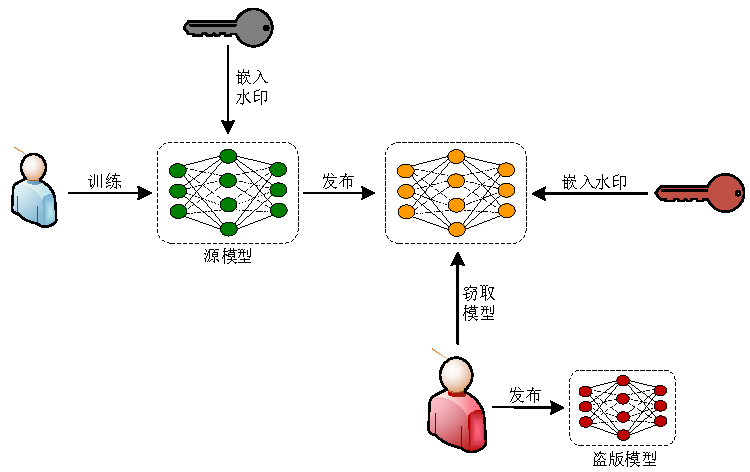
\includegraphics[width=1\linewidth]{歧义攻击示意图.pdf}
	\caption{歧义攻击示意图}
	\label{歧义攻击示意图}
	%	\vspace{-3mm}  %调整图片标题与下文距离,与\setlength{\belowcaptionskip}{-3mm}等效。
	\end {figure}	

如图\ref{歧义攻击示意图}所示,模型所有者在训练完源模型后,为了保护自己的知识产权,给DNN模型嵌入水印,然后发布公开服务。模型盗窃者访问公开的模型或者API,通过一定的方法复制篡改而得到盗版模型。为了躲避模型所有者的检测,盗窃者不关心原有的水印,而是给模型嵌入自己的额外水印,以此来混淆模型所有权的验证。

\begin{figure}[htbp]%%图,[htbp]是浮动格式
	\centering
	\setlength{\abovecaptionskip}{3mm} %图片标题与图片距离
	\vspace{-2mm}
	\setlength{\belowcaptionskip}{-3mm} %调整图片标题与下文距离
	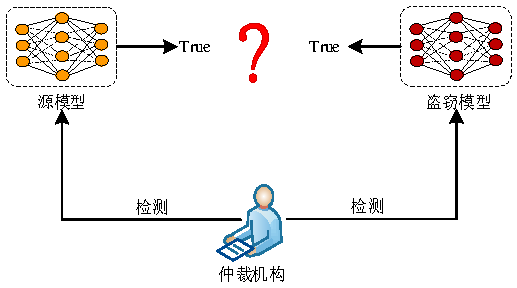
\includegraphics[width=0.8\linewidth]{检测歧义示意图.pdf}
	\caption{检测歧义示意图}
	\label{检测歧义示意图}
	%	\vspace{-3mm}  %调整图片标题与下文距离,与\setlength{\belowcaptionskip}{-3mm}等效。
	\end {figure}
	
如图\ref{检测歧义示意图}所示,模型所有者怀疑可疑模型是从自己的模型派生,向三方机构发起仲裁。仲裁机构进行模型所有者的水印检测,成功响应了嵌入的水印。于此同时,盗窃者的水印同样能够被检测出来,这种情况下无法进行正确的所有权决策。

具体来说,盗窃者对源模型嵌入新的水印或提取其他的指纹使原本的保护措施无效。歧义攻击对现有的深度神经网络模型的知识产权保护方法构成了严重威胁,在传统的数字水印领域中有研究表明,除非水印方案是不可逆的\cite{fan2019rethinking},否则鲁棒性的水印也不一定能验证所有权。

在本文中,我们认为通过验证可疑模型是否具有源模型特定的水印或指纹来讨论盗窃行为是不充分的,特别是出现歧义攻击时。因此我们提出推断模型所有权而不是验证,这是一种解决DNN模型所有权的新思路,与传统的通过模型水印和指纹验证所有权有所不同。这种方法的灵感来自于数据集推断\cite{maini2021dataset} 提出的所有权决策,我们将在下一小节中具体讨论。

\subsection{利用数据推断模型所有权}\label{4.1.2}

数据集推断做了一个假设:源模型的知识来自于训练数据集。无论盗窃模型是直接攻击源模型还是其副产品,盗窃模型的知识仍然是源模型中包含的知识。如果原始训练数据集是私有的,那么模型所有者在进行数据集推断时,相比盗窃者拥有强大的优势,因为源模型在原始训练数据中的性能要远远优于其他数据集。因此,模型所有者通过评估多个数据点到决策边界的距离和统计测试相结合,可以得到模型的所有权归属。

如图\ref{数据集推断原理图}所示,因为DNN模型是从数据集训练而来,所以模型中总会包含来自数据集中的知识。盗窃模型是从源模型派生,尽管包含的知识和源模型不可能完全相同,但总是有一部分是来自原始数据集,这是利用数据集做模型所有权推断的理论基础。

\begin{figure}[htbp]%%图,[htbp]是浮动格式
	\centering
	\setlength{\abovecaptionskip}{3mm} %图片标题与图片距离
	\vspace{-2mm}
	\setlength{\belowcaptionskip}{-3mm} %调整图片标题与下文距离
	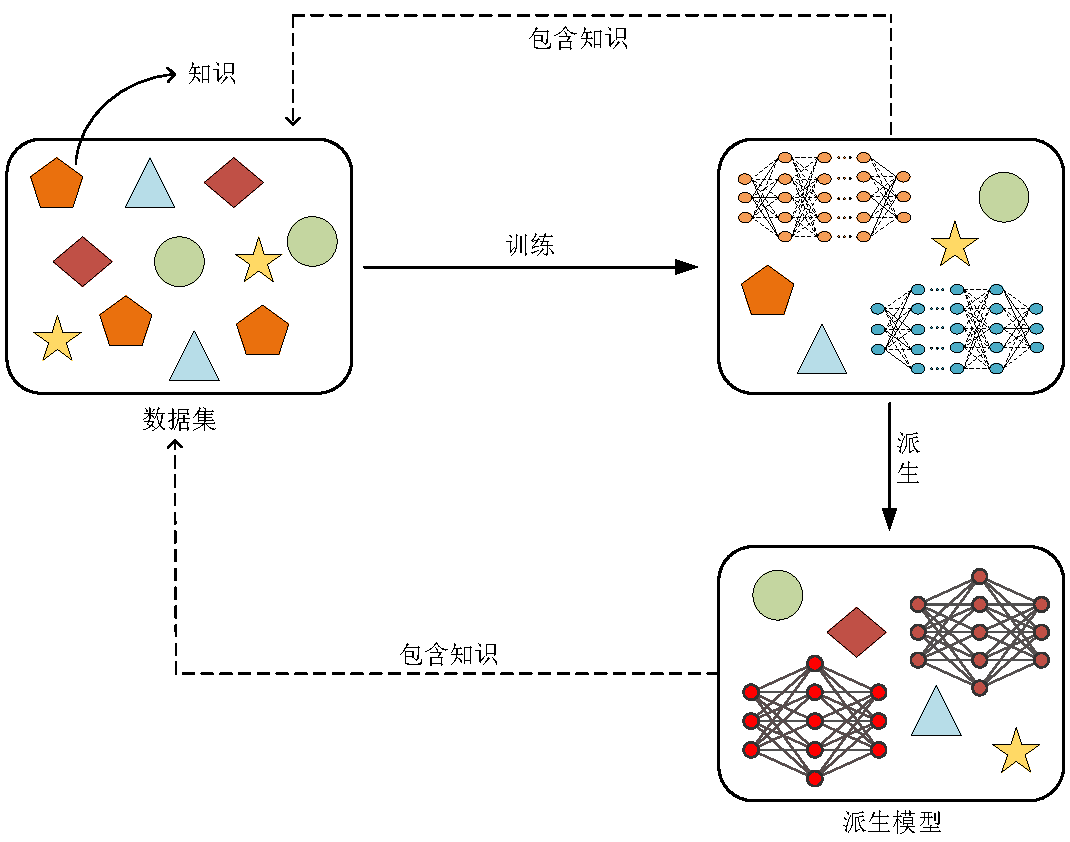
\includegraphics[width=0.8\linewidth]{数据集推断原理图.pdf}
	\caption{数据集推断原理图}
	\label{数据集推断原理图}
	%	\vspace{-3mm}  %调整图片标题与下文距离,与\setlength{\belowcaptionskip}{-3mm}等效。
	\end {figure}	
	
模型窃取过程中,源模型中的知识会传播到盗窃模型,使得所有盗窃模型总是包含一部分源模型训练数据集中的直接或间接信息。利用数据集做模型所有权推测和传统的验证模型所有权不同,通过私有数据集推断得到的是一个所有权决策,其中决策的最大者被认为拥有所有权。传统的模型所有权验证是从模型中提取水印或指纹进行匹配从而验证,这里涉及到了歧义攻击导致的验证冲突。从决策过程可以发现数据集推断得到的是一个“最”的概念,模型的所有权归属于决策指标的最大者,而不是进行类似模型水印和指纹的特定响应匹配,因此可以有效避免歧义攻击。

本文的工作是受到数据集推断验证模型所有权的启发,我们提出使用数据驱动推断模型所有权代替验证所有权。所有权推断可以在有效证明所有权归属的同时,解决所有权验证冲突的问题。除此之外,数据驱动的推断所有权意味着该方法只和DNN模型的输入输出相关,那么本文提出的方法既可以在白盒环境也可以在黑盒环境下工作。

利用数据推断模型所有权为保护模型知识产权提供了一个新的方向,但是目前数据集推断仍然具有以下\textbf{局限性}:

1)使用数据集推断的前提是原始训练数据不能被盗窃者获得,所以公开的数据集不能被用于训练源模型。然而,在大多数真实场景下,只有很少一部分工作会构造私有数据集用于训练模型,甚至这部分工作只应用于特定的领域中,这也意味着模型被盗窃的风险较小。因此,依赖于私有数据集的数据集推理方法在实际应用中使用范围很小,不能被大幅度推广使用。

2)数据集推理方法的核心思想是源模型的功能在训练数据上的效果优于其他数据,但是存在模型的功能可能相似,而结构和训练数据都不同的情况,因此该方法的结果可能会导致错误,将不相关模型判定为盗窃模型。Li等人\cite{lao2022deepauth}验证了这个局限性,表明在此种情况下该方法产生的结果值得怀疑。


因此,利用数据推断所有权的方法需要解决以上问题。在\ref{3}中,我们提出了近边界数据的概念,研究了它的近边界特性和类似对抗性样本可以转移到派生模型上特点,本文提出的方法将基于近边界数据推断DNN模型所有权。针对现有的数据集推断方法存在的问题,主要有以下的两点改进:

1)我们在公开数据集上生成近边界对抗性样本,并且通过训练生成对抗网络生成私有化的近边界数据,在解决数据集推断只能用于私有数据集问题的同时,也防止了本文的近边界数据被轻易复制和模仿,保留私有近边界数据在推断模型所有权时的优势。

2)本文的方法利用近边界数据靠近决策边界的特性解决模型功能相似引起的误导。这是因为即使模型功能相似,但是决策边界不可能完全相同,如果近边界数据在可疑模型上并没有表现出近边界性,那么不会判定该模型是盗窃模型。

下一节中,我们将详细讨论本文基于近边界数据的模型所有权推断方法,包括方法的设计目标,详细的执行流程和对方法产生结果的假设检验。

\section{近边界数据推断模型所有权}\label{4.2}

在本文中,我们提出了近边界数据,一种分布在分类边界附近的特殊样本。模型指纹\cite{cao2021ipguard}使用对抗性样本抽象地反映模型分类边界,同一组对抗性样本的输入,其引起的决策模式的变化可以用于比较模型知识的相似性,但这种方法是脆弱的,一般的模型窃取攻击都会修改源模型,而对模型的任意修改操作都有可能破坏这种特性。因此,我们不直接比较决策模式的变化,它是不可信任的,而是比较对抗性样本与决策边界的距离。大多数对抗性样本都是位于决策边界附近的,也就是说,它们与决策边界的距离很近。对抗性样本的这种性质被我们所利用并构造近边界数据,经过测试我们发现绝大多数的模型窃取方法都无法改变这种结果,即使样本分类被影响,其仍然位于分类边界附近。

近边界数据背后的意义是数据的近边界特性不会因为受到模型窃取攻击产生的模型修改而消失。受到这个特点的启发,将近边界数据作为水印验证所有权是传统的思路,虽然不会对模型的精度造成影响,但是这样的水印是脆弱的,很容易受到御歧义攻击,因此我们提出由近边界数据驱动的所有权推断方法,方法的主要原理如图\ref{方法原理图}所示。

\begin{figure}[htbp]%%图,[htbp]是浮动格式
	\centering
	\setlength{\abovecaptionskip}{5mm} %图片标题与图片距离
%	\vspace{-2mm}
	\setlength{\belowcaptionskip}{-3mm} %调整图片标题与下文距离
	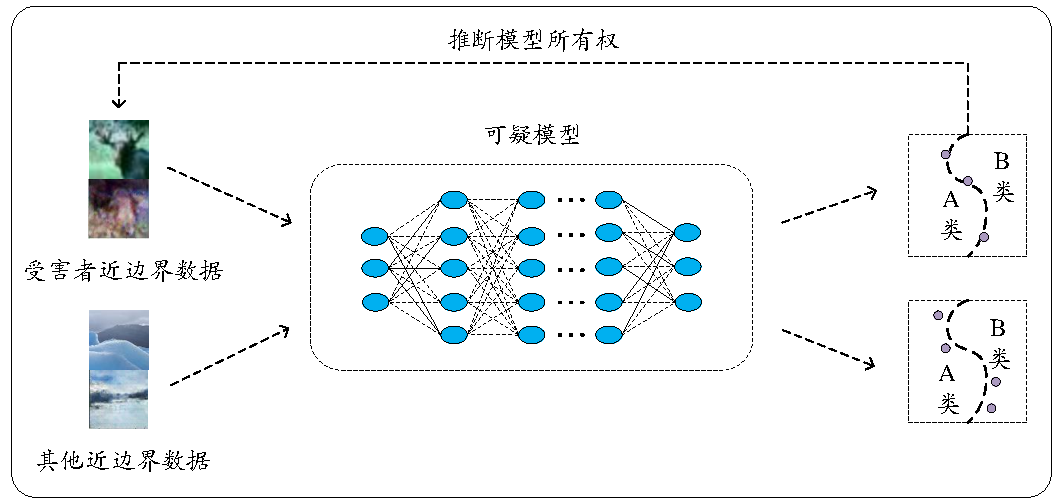
\includegraphics[width=0.97\linewidth]{方法原理图.pdf}
	\caption{近边界数据推断所有权}
	\label{方法原理图}
	%	\vspace{-3mm}  %调整图片标题与下文距离,与\setlength{\belowcaptionskip}{-3mm}等效。
	\end {figure}
	
如图\ref{方法原理图}所示,本文提出方法的主要思想是构造私有的近边界数据,以数据驱动推断模型的所有权。当模型所有者怀疑可疑模型是盗窃自己的模型时,向三方机构发起仲裁。模型所有者和可疑对手分别提供各自的私有近边界数据,仲裁机构分别计算双方数据的输出结果,统计测试样本数据点到分类边界的距离,距离近的判定获得模型所有权。

\subsection{设计目标}

依据现有的工作,本文提出的的方法在源模型训练后进行部署,且在黑盒环境下推断模型所有权。我们的方法不关注模型被盗窃的过程,而是聚焦在准确地推断DNN模型的所有权和识别不法分子的模型盗窃行为。现在大多数所有权验证技术都是黑盒模型环境,黑盒模式的适用情况更加广泛,因为模型所有者和攻击者通常不会提供完整模型,而是以API的形式提供商业服务。本文提出的方法仅利用模型提供的外部API,获取近边界数据的决策结果,从而推断模型所有权。

在通常的假设中,存在一个官方的仲裁机构,当对任一模型产生所有权怀疑时,受害者和可疑对手可以向机构提出申请并提供各自的私有化近边界数据,并通过我们的方法推断所有权。注意无论是在白盒的环境还是在黑盒的环境下,本文提出的方法均可以用来推断模型所有权。

本文提出的方法需要成功推断模型所有权,与此同时,需要保持DNN模型的性能并且不能对无关模型产生错误的所有权误导。因此本文提出方法的设计目标如下:

1)\textbf{精确性:}推断模型所有权的方法不应该影响模型的性能,模型的最大可接受测试精度下降不超过3\%。为了增加推断成功的置信度,在生成私有近边界数据后,我们会利用近边界数据微调源模型,使私有的近边界数据更加靠近分类边界。但是这不应该对模型的性能造成很大的影响,可以接受的精度下降不超过3\%。

2)\textbf{可转移性:}如果可疑模型与源模型相同或从源模型派生而来,则私有近边界数据在这些模型中均表现出近边界性。反之,近边界数据在无关模型中没有明显特征,防止产生所有权推断误导。

3)\textbf{有效性:}如果可疑模型与源模型相同或从源模型派生而来,则根据源模型构造的私有近边界数据在这些模型中距离指定的分类边界最近,这是本文方法能成功推断模型所有权的依据。

4)\textbf{鲁棒性:}近边界数据应该对常见的模型修改(如模型微调、剪枝和有损压缩)具有鲁棒性,这是本文方法能广泛应用的关键。

5)\textbf{不可见性:}敌手无法获得私有的近边界数据,也无法在视觉上观察到近边界数据的部署。

6)\textbf{高效性:}通过近边界数据推断模型所有权应该能够高效地计算距离边界数据,并通过对比全部近边界数据的决策结果确定可疑模型是否是盗窃模型。


\subsection{方法概述}

为了实现以上目标,本文提出了一种基于近边界数据的模型所有权推断方法。首先从训练数据集中生成近边界对抗性样本,接着训练生成对抗模型生成私有化近边界数据,然后使用私有化近边界数据微调源模型,最后对模型输出结果进行假设检验比对结果。

\noindent\textbf{问题定义:}我们定义了一个深度神经网络(DNN)分类器$G$作为源模型,给定一个原始训练集$D$,假设该源模型是一个$n$-类的DNN分类器,分类器的输出层为softmax层或其他决策层,决策函数$g_j(x)$表示数据样本$x$被分到第$j$类的概率,其中$j$ = 1,2,..,$n$。$Z_1$,$Z_2$,..,$Z_n$表示模型分类器的全部决策函数输出,其结果可作为分类边界的依据被我们使用,因此

\begin{equation}
	g_j(x) = \frac{exp(Z_j(x))}{\sum_{i = 1}^n exp(Z_i(x))}
\end{equation}

\noindent 其中,数据样本$x$的标签$y$被推断拥有最大概率的类别,例如$y = arg \mathop{max} \limits_j g_j(x) = arg \mathop{max} \limits_j Z_j(x)$。

通常来说,寻找位于分类边界上的数据点采用重复随机采样数据点的方法,如果数据点满足定义\ref{def:1},那么数据点位于分类边界上。然而,简单的重复采样可能需要大量的时间消耗,甚至无法找到这样的数据点。为了解决这个的问题,我们在\ref{3}中讨论了如何构造位于分类边界上或其附近的的数据点,且将其私有化的过程。

基于前面的讨论,模型窃取攻击通常来说会对模型进行修改,无法保证位于源模型分类边界上的点依旧位于盗窃模型分类边界上。因此,本文提出了鲁棒性更强的近边界数据的概念,它与对抗性样本类似,近边界特点可以转移到源模型派生出的模型上。近边界数据的优势在于它是到分类边界距离的衡量,即使对模型修改后,分类边界发生了一定的偏移,仍然可以计算近边界数据到分类边界的距离。本文的方法建立在\ref{3}研究的近边界数据之上。

本文提出构造私有化近边界数据推断模型的所有权,而不是验证所有权。本文方法的整体流程如图\ref{方法流程图}所示。

\begin{figure}[htbp]%%图,[htbp]是浮动格式
	\centering
	\setlength{\abovecaptionskip}{5mm} %图片标题与图片距离
	\vspace{-1mm}
	\setlength{\belowcaptionskip}{-3mm} %调整图片标题与下文距离
	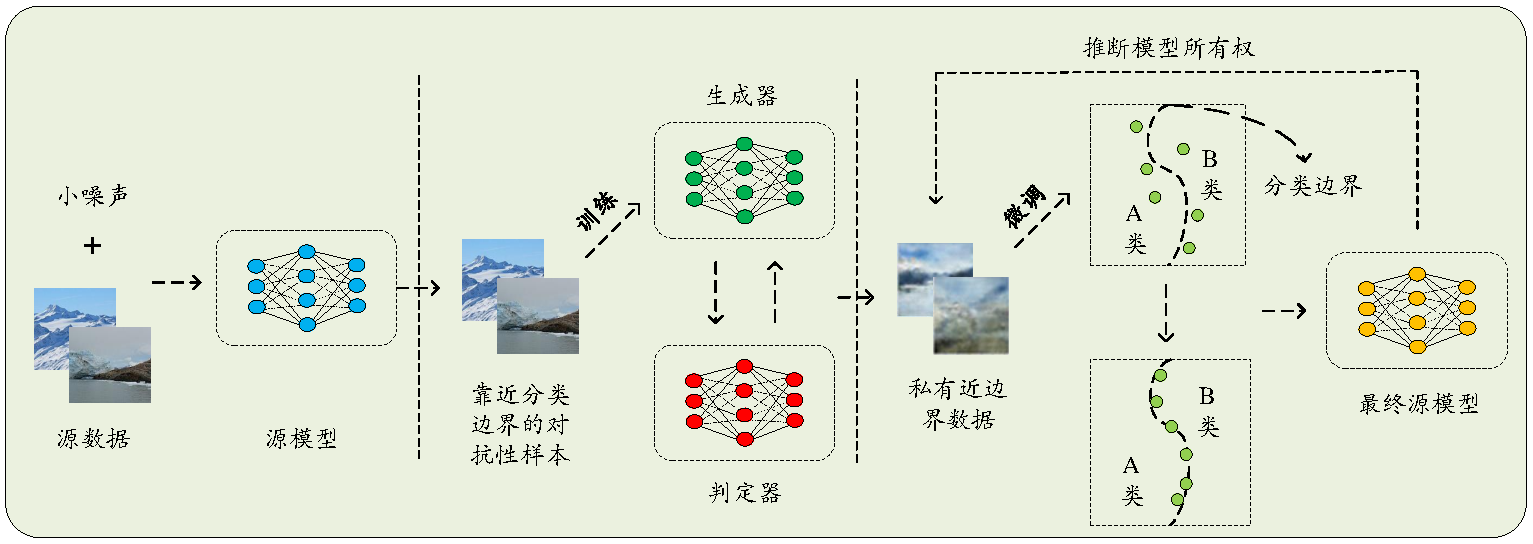
\includegraphics[width=1\linewidth]{方法流程图.pdf}
	\caption{方法整体流程图}
	\label{方法流程图}
	%	\vspace{-3mm}  %调整图片标题与下文距离,与\setlength{\belowcaptionskip}{-3mm}等效。
	\end {figure}
		
在图\ref{方法流程图}中,主要包含三个阶段:

1)从公开数据集中生成近边界对抗性样本。由于自然的近边界数据在样本空间中非常的少,甚至可以忽略不计,因此我们从众多生成对抗性样本的算法中测试并挑选了CW-$L_2$作为基础算法。并且在此基础上在算法中引入到分类边界距离这一衡量尺标,仅仅在距离变小时更新样本和距离参数,在距离小于预定阈值时提前终止算法。有效提升了生成近边界对抗性样本的质量和算法的效率。

2)训练生成对抗模型生成私有化的近边界数据。本文的的算法原理是模型所有者和可疑对手分别提供近边界数据输入可疑模型计算到分类边界的距离,距离小的获得模型所有权。大多数模型的训练使用的都是公开数据集,可疑对手可以采用相同的方法构造近边界数据。如果近边界数据被可疑对手轻易的复制,那么所有者的近边界数据在进行所有权推断时就失去了优势。因此,本文使用生成对抗网络学习近边界数据的特征,然后使用生成器私有化近边界数据,防止可疑对手轻易地模仿复制。

3)使用近边界数据微调源模型。使用生成对抗模型私有化近边界数据后,由于随机因素,相比于直接生成的近边界数据,私有化的近边界数据到分类边界距离可能会变大。因此我们设计了新的损失函数和训练方式来微调源模型,在保持模型性能的情况下,使私有化的近边界数据更加靠近分类边界,以此来提高模型所有权推断的置信度。

\subsection{假设检验}\label{4.2.3}

根据上一节的讨论结果,本文认为过去的验证模型所有权的思路具有较大的局限性,大多数研究无法抵御歧义攻击。因此,我们提出了推断模型所有权的想法,这是一种“最”的思路。在现实情况中,我们假设存在第三方仲裁机构,并约定目标分类边界,被盗窃者向第三方机构提出仲裁并提供近边界数据,盗窃者同样需要提供相应的近边界数据,第三方机构分别计算目标分类边界距离,本文认为持有最靠近目标分类边界的近边界数据所有者将获得模型所有权。注意,由于近边界数据通常是一组数据,所以应该根据统计的结果来看。在实验中,我们计算了不同规模的近边界数据组在源模型, 盗窃模型以及不相关模型上到分类边界的距离,并设计了一种基于假设检验的方法来表现推断的置信度。

\noindent\textbf{假设检验:}我们假设事件$C$是模型所有者提供的私有近边界数据在可疑模型上的计算结果,事件$C_S$ 表示盗窃者提供的近边界数据在可疑模型上的计算结果,或模型所有者提供的私有近边界数据在无关模型上的计算结果。本文计算假设$H_0:\mu \geq \mu_S(H_1:\mu < \mu_S)$的$p$值,以及差异大小$\Delta \mu = \mu_S - \mu$,$\Delta\mu$越大,推断可信度越高。如果$p$值低于预定义的置信度评分$\alpha$,则拒绝$H_0$,并称正在测试的模型是被盗模型。我们重复30次统计性实验以提高可信度。

假设检验的具体过程如算法\ref{alg:4}所示。

\begin{algorithm}[h] 
	\setstretch{1.2}
	\caption{假设检验}
	\label{alg:4}
	\begin{algorithmic}[1]
		
		\Require 模型所有者私有近边界数据样本$X$;可疑对手近边界数据样本$X_S$;可疑模型$\tilde{M}$;假设检验对照表$T$;显著性水平$\alpha$
		\Ensure 可疑模型是否为盗窃模型
		\State 原假设:$H_0:\mu \geq \mu_S$
		\State 备择假设:$H_1:\mu < \mu_S$
		\State 计算模型所有者私有近边界数据样本均值$\overline{X}$                     
		\State 计算可疑对手近边界数据样本均值$\overline{X}_S$ 
		\State 计算统计量$t$
		\State 查对照表$T$获得临界值$\lambda$
		\If{$t > \lambda$}
		\State $p < \alpha$,拒绝$H_0$,接受$H_1$,可疑模型是被盗模型
		\Else \State $p > \alpha$,不拒绝$H_0$
		\EndIf
	\end{algorithmic}
\end{algorithm}

\section{本章小结}

本章主要描述了本文提出的基于近边界数据的模型所有权推断方法。首先介绍了该方法的理论驱动,接着针对现有方法存在的问题提出本文方法的设计目标,即精确性、可转移性、有效性、鲁棒性、不可见性和高效性。然后对实现方法做了概述,并介绍了该方法的主要流程:从数据集样本中生成对抗性样本,训练生成对抗模型私有化近边界数据和使用近边界数据微调源模型。最后,提出了使用假设检验的方法来对模型所有者和可疑对手的输出结果进行比对,推断模型所有权。
